%% EXHALE method paper -- scaffold/draft.
%% Class: AASTeX v7.0.1 (aastex701.cls, 2025/05/09), included in this folder.
\documentclass[twocolumn]{aastex702}

\usepackage{booktabs}
\usepackage{amsmath}

\newcommand{\EXHALE}{\texttt{EXHALE}}
\newcommand{\ATES}{\texttt{ATES}}
\newcommand{\AIOLOS}{\texttt{AIOLOS}}
\newcommand{\Rp}{R_{\rm p}}
\newcommand{\Rstar}{R_{\star}}
\newcommand{\Mdot}{\dot{M}}
\newcommand{\Fxuv}{F_{\rm XUV}}
\newcommand{\HeTS}{\mathrm{He}\,2^{3}S}
\newcommand{\Lya}{\mbox{Ly}\ensuremath{\alpha}}
\newcommand{\Ha}{\mbox{H}\ensuremath{\alpha}}

\shorttitle{EXHALE: escaping exoplanet atmospheres}
\shortauthors{Seon}

\begin{document}

\title{EXHALE: A 1-D Multi-frequency Photoionization--Hydrodynamics Model of
Escaping Exoplanet Atmospheres}

\author{Kwang-Il Seon}
\affiliation{Korea Astronomy and Space Science Institute (KASI)} % TODO confirm affiliation line
\email{kwangil.seon@gmail.com} % v7 requires an email per author

\begin{abstract}
We present \EXHALE, a one-dimensional, multi-frequency photoionization--hydrodynamics
model for the XUV-driven escape of close-in exoplanet atmospheres and for the
transit-absorption diagnostics that trace it. \EXHALE\ evolves the compressible Euler
equations for a single bulk fluid on a spherical grid with a Godunov finite-volume
scheme (HLLC/Roe fluxes, PLM and WENO3 reconstruction) and relaxes to a stationary
transonic wind, with an optional Jacobian-free Newton--Krylov (JFNK) solver that drives
the discrete steady residual to machine-relevant levels. The thermal and ionization
state is set by a coupled nonlinear system for hydrogen, helium, and the trace metals
C, N, O, Mg, Ca, Na, and Fe, solved with an analytic-Jacobian Newton iteration and a
MINPACK fallback, using Badnell radiative and dielectronic recombination, Voronov
collisional ionization, and Kingdon \& Ferland charge exchange with hydrogen. Cooling
includes \Lya, recombination, free--free, and closed-form metal-line coefficients fitted
to CHIANTI. \EXHALE\ solves the metastable $\HeTS$ population that produces the
\mbox{He\,\textsc{i}} 10830~\AA\ triplet, builds the non-LTE $n=2$ hydrogen population
for the Balmer lines with an in-line \Lya\ escape-probability radiative-transfer field,
allows diffusive He/H (and He/metal) separation, and can adopt a lower-atmosphere base
from a photochemical (\texttt{VULCAN}) column. We apply the model to HD~209458~b,
HD~189733~b, WASP-52~b, and WASP-121~b and compare synthetic \mbox{He\,10830}, \Ha,
\Lya, and metal-line transit depths against published observations. The four
Newton-converged models span mass-loss rates
$\log_{10}(\Mdot/{\rm g\,s^{-1}})\approx9.0$--$13.2$, from the compact
HD~189733~b wind to the strongly irradiated WASP-121~b, with thermosphere
temperature maxima of $\sim0.8$--$1.2\times10^{4}$~K. The
synthetic depths range from sub-percent \Ha\ on the quieter targets to tens of
percent in \mbox{He\,10830} and \Lya, and are compared line by line with
published measurements; the model reproduces the order of magnitude of the
observed \mbox{He\,10830}, \Ha, and \Lya\ absorption on the two cooler targets,
over-predicts the WASP-52~b depths, and on WASP-121~b saturates against the
truncation of the modeled domain, motivating the composition and
domain refinements discussed in the text.
\end{abstract}

\keywords{planets and satellites: atmospheres --- hydrodynamics ---
radiative transfer --- methods: numerical}

%=====================================================================
\section{Introduction}
\label{sec:intro}
%=====================================================================

Close-in giant planets receive intense stellar X-ray and extreme-ultraviolet (XUV)
irradiation. Photoionization deposits energy in the upper atmosphere, heats it to
$\sim10^4$~K, and drives a transonic hydrodynamic wind that carries mass away from the
planet \citep{Parker1958,MurrayClay2009}. This escape sculpts the mass--radius
distribution of the exoplanet population and can be observed directly through excess
absorption in a handful of spectral tracers during transit.

Four diagnostics dominate the observational picture. The \mbox{He\,\textsc{i}} 10830~\AA\
triplet arises from the metastable $\HeTS$ level, which is populated by recombination of
\mbox{He\,\textsc{ii}} and depopulated by photoionization, radiative decay, and
collisions; because the mid-ultraviolet flux that photoionizes $\HeTS$ and the XUV flux
that produces \mbox{He\,\textsc{ii}} depend on the host star, the 10830 line is a sensitive
probe of both the wind structure and the stellar spectrum
\citep{OklopcicHirata2018,Yan2022}. The hydrogen Balmer lines, chiefly \Ha, absorb from
the $n=2$ level, whose population is set primarily by \Lya\ radiative pumping and thus
requires a resonant-line radiative-transfer treatment \citep{Christie2013,Huang2017}.
\Lya\ itself is a strong but interstellar-absorbed tracer of neutral hydrogen. Finally,
metal resonance lines (\mbox{Mg\,\textsc{ii}} h\&k, \mbox{Ca\,\textsc{ii}} H\&K,
\mbox{Na\,\textsc{i}} D, and \mbox{Fe\,\textsc{ii}}) probe the ionization and thermal
structure of the wind and, for the hottest planets, its metal content
\citep{Huang2023,Koskinen2022}.

A number of one-dimensional escape models have been built to interpret these tracers,
spanning steady-state boundary-value solvers \citep{MurrayClay2009}, time-relaxation
photoionization-hydrodynamics codes \citep{Salz2016,Caldiroli2021}, grid-production
schemes \citep{Kubyshkina2018}, and dedicated multispecies thermosphere models with
excited-state microphysics \citep{Taylor2025,Taylor2026}. \EXHALE\ belongs to this last,
diagnostic-oriented family. It began as a fork of the \ATES\ photoionization
hydrodynamics code \citep{Caldiroli2021,Caldiroli2022} and retains its Godunov hydro
core and boundary/initial-condition skeleton, while adding a coupled trace-metal
ionization network with self-consistent equation of state, CHIANTI metal-line cooling,
the $\HeTS$ metastable network, the non-LTE $n=2$ hydrogen population with in-line \Lya\
radiative transfer, diffusive He/H separation, a direct steady-state (JFNK) solver, and
a tiered coupling to the lower atmosphere. This paper documents the physics and numerics
of \EXHALE\ and applies it to four benchmark planets.

Section~\ref{sec:method} describes the model. Section~\ref{sec:ates} contrasts \EXHALE\
with \ATES\ in both algorithm and physics. Section~\ref{sec:results} presents the
application to each planet (scaffold), and Section~\ref{sec:summary} summarizes.

%=====================================================================
\section{Method}
\label{sec:method}
%=====================================================================

\subsection{Hydrodynamics and numerical scheme}
\label{sec:hydro}

\EXHALE\ solves the one-dimensional, spherically symmetric Euler equations for mass,
radial momentum, and total energy of a single bulk fluid, with source terms for gravity,
tidal (Roche) and centrifugal forces, photoionization heating, and radiative cooling.
The discretization is a finite-volume Godunov method inherited from \ATES: fluxes are
computed with an approximate Riemann solver (HLLC by default; Roe and local
Lax--Friedrichs are also available), the interface states are reconstructed either with a
piecewise-linear method (PLM, MC-limited) or with a third-order essentially
non-oscillatory scheme (ESWENO3), and time integration uses a strong-stability-preserving
Runge--Kutta update at CFL number $0.6$ \citep{Caldiroli2021,Salz2016}. The grid has 500
cells plus ghost cells on a mixed uniform--stretched mesh spanning the base radius to the
outer boundary. The spacing of the uniform region is a runtime quantity, because it sets
the number of cells per base density scale height $H=k_BT/(\mu g)$, and a base resolved by
too few cells supports a stationary cell-to-cell entropy (contact) mode that the
non-dissipative Riemann fluxes do not damp. The code reports $H(T_{\rm eq})/\Delta r$ at
startup; on the default grid this is $\approx27$ cells for HD~189733~b against
$\approx102$ for WASP-121~b, and the high-gravity, compact HD~189733~b is correspondingly
the planet of the four that needs a refined base. In this respect \EXHALE\ and the
PLUTO--CLOUDY interface of
\citet{Salz2016} are numerical near-twins, sharing the same reconstruction, Riemann
solver, and time integrator.

The stationary transonic wind is reached in two complementary ways. The default is time
relaxation, converged on the spatial flatness of the mass flux
$\rho v r^2$ over the wind window,
\begin{equation}
du \;=\; \frac{\max_j |\rho v r^2|_j - \min_j |\rho v r^2|_j}
              {\min_j |\rho v r^2|_j} \;<\; du_{\rm th},
\end{equation}
with a two-stage schedule that marches first with PLM (robust) and then with WENO3
(low-diffusion) to a final tolerance $du_{\rm th}=10^{-3}$. This mass-flux criterion has
two known blind spots: it cannot detect a uniform level drift of an already-flat profile,
and on the strongly driven planets it dips transiently below threshold long before the
wind settles, so a premature snapshot can be reported as steady. \EXHALE\ therefore adds
(i) a level-stability gate on the windowed mean of $|\rho v r^2|$ and (ii) a diagnostic
that evaluates the finite-volume steady residual $\mathbf{R}$ directly (mass, momentum,
and heating-minus-cooling energy balance), which ranks candidate states independently of
$du$ and can serve as the convergence test.

For quantitative mass-loss rates \EXHALE\ provides a direct steady-state solver that
finds the root of the discrete residual, $F(Y)=0$, where $Y=(\rho,\rho v,E)$ on the
physical cells and the ionization equilibrium (with its heating and cooling) is
eliminated locally inside every residual evaluation. The nonlinear system is solved by
pseudo-transient-continuation Newton iteration with an inexact Jacobian-free
Newton--Krylov (JFNK) inner solve: a banded finite-difference Jacobian, obtained from a
graph-colored stencil and factored with LAPACK, preconditions a matrix-free GMRES whose
Jacobian--vector products capture the weakly non-local radiation response. Robust
convergence required a smooth $\ell_2$ line-search merit, diagonal scaling across the
several decades spanned by the base-to-wind density contrast, a differentiable base
velocity valve, frozen WENO smoothness weights during the
inner solve, and a non-monotone (Grippo) step acceptance. The solver reaches steady
residual levels unattainable by time marching at a small fraction of the cost; a
best-iterate/fail-fast guard falls back to plain marching if the Newton basin is not
reached, so an unconverged state cannot be mistaken for the answer.

The lower boundary is a fixed reservoir. Density and temperature are held at the base
radius (total $n\sim10^{14}\,{\rm cm}^{-3}$ near a $\mu$bar pressure level, $T$ at the
planet's equilibrium value), and the ghost-cell velocity uses a one-way valve
$v_{\rm gh}=\max(v_1,0)$ that admits wind-feeding inflow but suppresses the base
oscillations (``breathing'') that otherwise develop at steep base density gradients ---
the same valve adopted independently by \citet{Caldiroli2021} and \citet{Salz2016}.
\EXHALE\ adds a dynamic base-pressure correction that pins the base temperature exactly
through the equation of state, and, for the Newton solver, a smooth variant of the valve.
The upper boundary is supersonic free outflow, imposed by zero-gradient or linear
extrapolation at the outer (Roche-lobe) radius. Within physically realistic ranges the
mass-loss rate is insensitive to the base density, temperature, and ionization fraction
but scales steeply with the base radius, $\Mdot\propto\Rp^3$
\citep{MurrayClay2009,Salz2016}; \EXHALE\ therefore treats the base radius (the pressure
level it corresponds to) as the physically important lower-boundary quantity.

\subsection{Photoionization, heating, and multi-frequency radiation}
\label{sec:photoion}

The stellar XUV field is attenuated radially and drives photoionization and
photoelectric heating. \EXHALE\ integrates each species' energy-dependent
photoionization cross section against the local stellar spectrum on a fixed energy grid.
The spectrum may be read as a two-column (wavelength, flux) file --- for example a
MUSCLES spectral energy distribution scaled to the orbital distance \citep{France2016} ---
or represented as a broken power law over an EUV band and an X-ray band normalized to the
band luminosities. Because the one-dimensional model is spherically symmetric and cannot
resolve the day--night illumination geometry, the ionizing flux entering the
hydrodynamics is reduced by a redistribution factor (the ``Rate/2 + Mdot/2''
approximation), valid as an average over the irradiated hemisphere; diagnostics that
model the one-sided illumination explicitly (e.g.\ the \Lya\ transfer of
Section~\ref{sec:hets}) instead use the full incident flux, to avoid double-counting the
geometry.

The photoionization cross sections combine exact and fitted forms. Hydrogen and
\mbox{He\,\textsc{ii}} use the analytic hydrogenic cross section with the Gaunt-factor
correction, exact at threshold ($6.3/Z^2$~Mb). The \mbox{He\,\textsc{i}} ground state
uses the single-shell analytic fit of \citet[VFKY96]{Verner1996} by default, which agrees
with the legacy two-term \ATES\ fit to within $14\%$ over $24.6$--$500$~eV; the metals
and \mbox{He\,\textsc{ii}} use the same VFKY96 functional form. The metastable $\HeTS$
level --- the lower state of the 10830 triplet, whose threshold lies at $4.77$~eV in the
mid-ultraviolet --- is not in the Verner tabulation, so it is represented by two VFKY96
terms (the $2s$-shell channel and the resonance-averaged \mbox{He\,\textsc{ii}} $n=2$
channel) joined by a log-linear bridge across the Cooper minimum. This construction
reproduces the Norcross (1971) tabulation shipped with \texttt{p-winds}
\citep{dosSantos2022} to within $\sim10\%$ and an independent TOPbase/Opacity Project
R-matrix cross section to within $\sim8\%$ in the smooth near-threshold region. The
autoionizing resonances that TOPbase resolves above $\sim35$~eV, and the smooth
high-energy tail above the fitted cutoff, each change the $\HeTS$ photoionization rate by
only $1$--$2\%$; because these are below the fit and composition uncertainties, they do
not affect the 10830 prediction (a documented approximation valid for the smooth
resonance-averaged background, which is what the broadband rate integral samples).

The energy deposited per photoionization is the photoelectron energy above threshold,
summed over every absorber the ionization network carries: \mbox{H\,\textsc{i}},
\mbox{He\,\textsc{i}}, \mbox{He\,\textsc{ii}}, the metastable $\HeTS$, and the
photoionizable trace metals (C, N, O, Mg, Ca, Na, and Fe ions); molecular runs add an
\mbox{H$_2$} photoionization term. The photoelectric heating efficiency is not unity: a
fraction of each primary photoelectron's energy drives secondary ionizations rather than
heating the gas, and \EXHALE\ reduces the deposited heat by that fraction following the
ionized-fraction partition of Shull \& van Steenberg (1985), applied as an optional,
staged activation, rather than treating the secondary ionizations as a separate channel.

Beyond the direct photoelectric heating, \EXHALE\ tracks four reprocessing channels that
return trapped line and recombination energy to the gas. Balmer-continuum photoelectric
heating draws on the excited $n=2$ hydrogen population \citep{Christie2013,Huang2017}.
\Lya\ de-excitation heating returns the $10.2$~eV excitation energy of \Lya-pumped $n=2$
hydrogen as heat when the level is collisionally de-excited, in the trapped-\Lya\ picture
of \citet{Huang2023}; the pumping field is the in-line \Lya\ transfer of
Section~\ref{sec:hets}. Helium recombination-coupling heating captures helium
recombination photons that photoionize and heat hydrogen. Finally, $\HeTS$+H
Penning-ionization heating uses the temperature-dependent rate of \citet{Taylor2025},
with a corresponding $\HeTS$+$\mathrm{H_2}$ term in molecular runs. The code writes each
of these heating terms, together with the direct photoionization heating of every
absorber, as a separate column of a diagnostic \texttt{Heating\_breakdown.txt} file whose
channel sum reproduces the total heating that enters the hydrodynamics
(Table~\ref{tab:energy}).

\subsection{Coupled ionization and thermochemistry}
\label{sec:ioniz}

The ionization state is computed in photoionization equilibrium as a single coupled
nonlinear algebraic system that includes hydrogen, helium, and the trace metals C, N, O,
Mg, Ca, Na, and Fe, each carried through its relevant ionization stages, together with
the metastable $\HeTS$ level and the excited $n=2$ hydrogen population. Solving all
species simultaneously (rather than element by element) captures the shared free-electron
density and the charge-exchange coupling between hydrogen and the metals. The system is
solved with an analytic-Jacobian Newton iteration and a MINPACK \texttt{hybrd1} dogleg
fallback for the cells where the Newton step leaves the physical region; the analytic
Jacobian carries the great majority of cells and the fallback guarantees robustness.

The reaction rates are drawn from standard atomic-data sources, not fitted internally:
radiative and dielectronic recombination from the Badnell data
\citep{Badnell2006rr,Badnell2003dr} (with Storey \& Hummer hydrogenic recombination where
appropriate; \citealt{StoreyHummer1995}), collisional ionization from the
\citet{Voronov1997} fits, and charge exchange between hydrogen and the metals from
\citet{KingdonFerland1996}, taken in the tabulation of \citet{Huang2023}. The
trace-metal abundances are set at runtime through a
configuration file, so a model can be run with or without metals without recompiling.
Because the metals contribute to the mass, electron, and particle budgets, they are
included self-consistently in the bulk-gas equation of state, so their presence feeds
back on the base density, pressure, and mean molecular weight rather than being a passive
overlay.

One entry of that tabulation is corrected here. As printed, the two oxygen rows of
Table~4 of \citet{Huang2023} are inconsistent with detailed balance: the
$\exp(-227/T)$ Boltzmann factor sits on the $\mathrm{O^+}+\mathrm{H}$ row, whereas
IP(\mbox{O\,\textsc{i}})~$=13.6181$~eV exceeds IP(\mbox{H\,\textsc{i}})~$=13.5984$~eV,
so that $\mathrm{O}+\mathrm{H^+}\rightarrow\mathrm{O^+}+\mathrm{H}$ is the endothermic
direction ($\Delta E/k = 227.7$~K, matching the printed argument to $0.3\%$) and is the
one that must carry it. Read as printed the pair violates detailed balance by a factor of
$1.47$ at $8000$~K; exchanging the two reactant labels restores it to within $9\%$. Both
the expressions of \citet{Huang2023} and the two oxygen fits carried by \textsc{Cloudy}
\citep{Cloudy2025} descend from the same calculation \citep{Stancil1999}, and the two
sources attach the labels the opposite way, agreeing to $1$--$3\%$ per direction under the
exchange; this is therefore a check of the assignment and not an independent
determination of the rate. Helium is the only other row of Table~4 carrying an explicit
Boltzmann factor whose placement is fixed by the ionization potentials, and it is printed
correctly, its argument $12.75$ (in units of $10^{4}$~K) matching
IP(\mbox{He\,\textsc{i}})~$-$~IP(\mbox{H\,\textsc{i}})~$=12.752$. The most likely reading
is therefore a transposition of the two oxygen labels rather than an error in the
coefficients, and we adopt the exchanged assignment. This concerns the printed table
only; we make no claim about the coefficients used in the calculations of
\citet{Huang2023}. In our WASP-121~b model the correction leaves the wind essentially
unchanged --- the mass-loss rate shifts by $0.05\%$ and the temperature by less than
$10$~K --- but it raises the neutral-oxygen density in the ionized wind by a factor of
$1.6$, which would matter for any \mbox{O\,\textsc{i}} line prediction.

\subsection{Cooling}
\label{sec:cooling}

The gas loses energy through several radiative channels, each of which \EXHALE\ writes as
a separate column of a diagnostic \texttt{Cooling\_breakdown.txt} file whose channel sum
reproduces the total radiative cooling. Collisional (line) excitation cooling is split by
absorber into an \mbox{H\,\textsc{i}} term --- dominated by \Lya\ and evaluated with the
CHIANTI-consistent form of \citet{Cen1992}, consistent with \citet{Black1981} --- and
separate \mbox{He\,\textsc{i}} and \mbox{He\,\textsc{ii}} terms. Collisional-ionization
cooling removes the ionization potential in each ionizing collision of \mbox{H\,\textsc{i}},
\mbox{He\,\textsc{i}}, and \mbox{He\,\textsc{ii}}. Radiative recombination cooling of
\mbox{H\,\textsc{ii}}, \mbox{He\,\textsc{ii}}, and \mbox{He\,\textsc{iii}} uses case-B
rates (Hui \& Gnedin 1997). Free--free (bremsstrahlung) emission scales as
$T^{0.55}\,n_e n_{\rm ion}$ and sums the contributions of hydrogen, helium, and the metal
ions, using the free--free Gaunt factor of van Hoof et al. The metastable helium level
contributes a $2^{3}S\to2^{3}P$ 10830 collisional-excitation cooling term. Metal-line
emission is treated as described next.

Metal-line cooling uses closed-form analytic coefficients fitted to the CHIANTI database
\citep{Dere1997,DelZanna2021} rather than large runtime tables. A single-channel
resonance line follows the exact two-level expression
\begin{equation}
\Lambda(T) \;=\; \frac{8.629\times10^{-6}}{g_l\,\sqrt{T}}\,
\Upsilon(T)\,\Delta E\,e^{-\Delta E/k_BT},
\end{equation}
with the slowly varying effective collision strength $\Upsilon(T)$ fitted in the
Burgess--Tully form; this reproduces the \mbox{Mg\,\textsc{i}}, \mbox{Mg\,\textsc{ii}},
\mbox{Ca\,\textsc{ii}}, and \mbox{Na\,\textsc{i}} D cooling to a few percent. Species with
many contributing transitions --- \mbox{Fe\,\textsc{ii}} and the C/N/O ions --- are
represented by a sum of effective two-level groups,
$\Lambda(T)=T^{-1/2}\sum_i A_i\,e^{-T_i/T}$, whose group temperatures map onto physically
distinct transition manifolds (infrared fine structure, optical metastable, ultraviolet
resonance, and a high-energy tail). These CHIANTI fits replace an earlier set of C/N/O
formulas inherited from \AIOLOS\ that omitted nitrogen entirely and deviated for oxygen
across the wind-launch temperature range; the fitted nitrogen cooling and corrected
oxygen curves are genuinely new physics rather than a re-parameterization.

For the ground-term fine-structure lines ([\mbox{C\,\textsc{ii}}] 158~$\mu$m,
[\mbox{O\,\textsc{i}}] 63~$\mu$m) the optically thin coronal limit overestimates the
cooling at the dense base, where the densities exceed the line critical densities. In
that regime the fine-structure floor is replaced by the exact two-level statistical
equilibrium solution, which saturates the line at high density and recovers the coronal
value in the low-density limit; this also restores the hydrogen-collision de-excitation
channel that the electron-only coronal curves omit. These two lines are additionally
allowed to be optically thick. Their line-center optical depth is accumulated over the
column between the emitting cell and the top of the domain, and the corresponding escape
probability $\beta(\tau)$ --- the plane-parallel Doppler form of \citet{HollenbachMcKee1979}
and \citet{deJong1980}, renormalized by a factor two so that $\beta(0)=1$ exactly, since
radiation escaping downward is absorbed by the lower atmosphere and leaves the modeled gas
either way --- multiplies the spontaneous rate, $A_{ul}\to\beta A_{ul}$, \emph{inside} the
two-level solution. Placing $\beta$ inside matters: in the subcritical limit the cooling is
fixed by the collisional excitation rate and must not depend on $\beta$, which an external
factor would violate. In the tenuous wind $\beta\to1$ and the optically thin result is
recovered; at the HD~189733~b base, where the layer is cold and dense,
$\tau([\mbox{O\,\textsc{i}}]\,63\,\mu{\rm m})\simeq3$ and the trapping is a factor of a few.
Resonance metal lines that can be thick in a metal-rich wind
(\mbox{Mg\,\textsc{ii}} h\&k) are still treated as optically thin; this is a documented
limitation rather than a solved problem.

All of the CHIANTI coefficients are fitted over $10^3$--$10^5$~K, and below that floor they
are not merely unvalidated but unphysical: their softest exponentials carry excitation
temperatures of several hundred to a few thousand kelvin that correspond to no ground-term
splitting of the ion in question. The coronal part is therefore removed smoothly below
$10^3$~K by a cutoff factor that is exactly unity at and above the floor, with continuous
value and temperature derivative (the bracketing temperature solve and the semi-implicit
energy update both differentiate the cooling in $T$). Only the explicit two-level
fine-structure terms, which are valid there, survive below the floor. The width of the
cutoff is a modeling choice, not a measurement. In molecular runs an $\mathrm{H_3^+}$
ro-vibrational cooling term is added (Miller et al. 2013).

The radiative channels above are the source term in the thermal energy equation; the gas
also loses energy dynamically. Adiabatic (expansion) cooling --- the $P\,dV$ work done by
the expanding wind --- is carried directly by the hydrodynamics rather than as a radiative
loss, and it is typically the dominant energy sink in the outer wind, where it becomes
comparable to or exceeds the radiative terms; the structure figures show it as a separate
curve. Thermal conduction and viscous dissipation are omitted by default: the viscosity
coefficient defaults to zero and thermal conduction is deferred, so neither enters the
present models. Table~\ref{tab:energy} collects all of the heating, cooling, and
dynamical channels together with their references.

\begin{deluxetable}{ll}
\tablecaption{Heating, cooling, and dynamical energy channels in \EXHALE. Each radiative
channel is written to a separate column of \texttt{Heating\_breakdown.txt} or
\texttt{Cooling\_breakdown.txt}, whose channel sums reproduce the total heating and
cooling that enter the hydrodynamics.\label{tab:energy}}
\tablehead{\colhead{Channel} & \colhead{Reference / form}}
\startdata
\cutinhead{Heating}
Photoionization, \mbox{H\,\textsc{i}} & photoelectron energy above threshold \\
Photoionization, \mbox{He\,\textsc{i}}, \mbox{He\,\textsc{ii}} & \\
Photoionization, $\HeTS$ metastable & mid-UV, $>4.77$~eV \\
Photoionization, C/N/O/Mg/Ca/Na/Fe ions & \\
Photoionization, $\mathrm{H_2}$ & molecular runs \\
Secondary-ionization efficiency reduction & Shull \& van Steenberg 1985 \\
Balmer-continuum photoelectric ($n=2$ H) & \citet{Christie2013,Huang2017} \\
\Lya\ de-excitation heating & \citet{Huang2023}; Sec.~\ref{sec:hets} \\
He recombination-coupling heating of H & \\
$\HeTS$+H Penning ionization & \citet{Taylor2025} \\
$\HeTS$+$\mathrm{H_2}$ Penning ionization & molecular runs \\
\cutinhead{Radiative cooling}
Collisional excitation, \mbox{H\,\textsc{i}} (\Lya) & \citet{Cen1992,Black1981} \\
Collisional excitation, \mbox{He\,\textsc{i}}, \mbox{He\,\textsc{ii}} & \\
Collisional ionization, H\,\textsc{i}/He\,\textsc{i}/He\,\textsc{ii} & \\
Radiative recombination (case B) & Hui \& Gnedin 1997 \\
Free--free, H + He + metal ions & van Hoof Gaunt factor \\
$\HeTS$ metastable $2^{3}S\to2^{3}P$ 10830 & \\
Metal lines, C/N/O/Mg/Ca/Na/Si/K/S/Fe & \citet{Dere1997,DelZanna2021} \\
$\mathrm{H_3^+}$ ro-vibrational & Miller et al. 2013; molecular runs \\
\cutinhead{Dynamical (energy equation)}
Adiabatic (expansion) cooling & $P\,dV$ work of the wind \\
Thermal conduction, viscous dissipation & omitted by default \\
\enddata
\end{deluxetable}

\subsection{The metastable helium triplet and in-line \Lya\ radiative transfer}
\label{sec:hets}

The \mbox{He\,\textsc{i}} 10830 and Balmer diagnostics require the excited-state
populations to be solved together with the wind. The metastable $\HeTS$ level is treated
as a separate species in the coupled system. In steady state its abundance relative to
\mbox{He\,\textsc{ii}} is
\begin{equation}
\frac{n(\HeTS)}{n_{\rm He^+}} \;\simeq\;
\frac{\alpha_3\,n_e}{\Phi_3 + A_{31} + (q_{31a}+q_{31b})n_e + Q_{31}n_{\rm H}},
\end{equation}
where $\alpha_3$ is the recombination rate into $2^3S$, $\Phi_3$ the mid-ultraviolet
photoionization rate, $A_{31}=1.27\times10^{-4}\,{\rm s}^{-1}$ the radiative decay, and
$q_{31}$, $Q_{31}$ the electron and hydrogen collisional sinks. The hydrogen-collision
sink includes the temperature-dependent Penning ionization rate of \citet{Taylor2025},
which replaces the older constant value and is often the dominant $2^3S$ loss near the
dense base.

The Balmer lines absorb from the $n=2$ hydrogen population, which is built following the
non-LTE rate equilibrium of \citet{Christie2013}: collisional excitation, recombination
cascade, two-photon decay, $\ell$-mixing between $2s$ and $2p$, and --- dominantly ---
\Lya\ radiative pumping $B_{1s\to2p}\bar{J}_{\Lya}$. Rather than a full Monte Carlo, which
is intractable at the \Lya\ line-center optical depths of a hot Jupiter
($\tau_0\sim10^{7}$--$10^{8}$, where core-skipping is both forbidden and incompatible with
the core-dominated pumping), \EXHALE\ evaluates $\bar{J}_{\Lya}$ from a local
escape-probability radiative-transfer field every time step. The treatment follows the
Neufeld/Harrington wing-escape solution, which is accurate in the very optically thick
limit $a\tau_0\gg1$ that applies here \citep{Neufeld1990}. It combines an internal source
term (recombination cascade plus electron-impact excitation) closed with the wing escape
probability $\beta=\pi^{-1/4}\sqrt{a/\tau}$ and a $(1-\beta)$ factor that prevents the
source function from diverging as the gas ionizes in the outer wind, plus a trapped
stellar-beam term whose penetration through the broad stellar-line wings uses the stellar
line width. An optional Sobolev (wind-velocity) escape term is included; for a hot Jupiter
it changes $\bar{J}_{\Lya}$ by less than a percent because the velocity gradient and the
\Lya\ opacity scale together. For percent-level \Ha\ work under one-sided illumination,
where the pumping field is only cylindrically symmetric, \EXHALE\ can instead ingest a
two-dimensional scattering-rate grid from the \texttt{LaRT} Monte Carlo code
\citep{SeonKim2020}.

\subsection{Diffusive separation}
\label{sec:diffusion}

Because helium is four times heavier than hydrogen, it is under-dragged by the escaping
hydrogen wind, so the escaping He/H ratio can fall below the bulk abundance with
increasing altitude. \EXHALE\ retains its single bulk-momentum formulation but represents
this separation with a molecular- plus eddy-diffusion term that lets the He/H ratio vary
with radius, in the spirit of \citet{Taylor2025} and consistent with the multi-fluid
result of \citet{Xing2023}. The homopause where the diffusive separation sets in is
controlled by an eddy-diffusion coefficient that can be supplied from the lower-atmosphere
model (Section~\ref{sec:lower}). The same framework extends to He/metal separation. This
altitude-dependent composition is what the transit post-processor requires for a
physically consistent \mbox{He\,10830} column; it is optional and off by default.

\subsection{Lower-atmosphere boundary}
\label{sec:lower}

The base of the escape model sits near a $\mu$bar pressure level, below which the
atmosphere is denser, cooler, and possibly molecular. \EXHALE\ couples to this region
through an optional handoff file (\texttt{base.inp}) that overrides the base temperature,
base radius, He/H ratio, and eddy-diffusion coefficient before the derived constants are
computed. A tiered set of lower-atmosphere models writes this file: an analytic
hydrostatic column that returns the $1\,\mu$bar radius and a molecular-hydrogen fraction;
a molecular-chemistry option with $\mathrm{H_3^+}$ cooling for genuinely cool
sub-Neptunes; and, at the most complete tier, a photochemical column from the
\texttt{VULCAN} code \citep{Tsai2017}, whose disequilibrium composition replaces the
chemical-equilibrium estimate \citep{Visscher2006,Moses2011}. For a warm hot Jupiter the
photochemical base dissociates far more hydrogen than chemical equilibrium predicts, so
the atomic base that the escape model assumes rests on photochemistry rather than on
thermal dissociation; \texttt{VULCAN}, however, does not release the atomic metals
(Na/Mg/Ca/Fe), whose abundances remain user-supplied.

The coupling is one-way by default (lower atmosphere $\to$ base $\to$ escape). Two
caveats bound its validity. First, the composition must not be double-counted: if the
handoff file sets the He/H ratio from the lower model, the metal abundances should be that
model's atomic-release values rather than solar totals. Second, and most important, the
handoff assumes that the base pressure lands below the thermospheric temperature rise. If
it instead falls inside a thermospheric temperature inversion --- where the escape model's
own heating has already raised the temperature --- then adopting a cool lower-atmosphere
$T$ and composition at that level double-counts the transition region and misrepresents
the base state. The handoff is therefore valid only when the chosen pressure level sits
beneath the onset of thermospheric heating; for dayside-hot or strongly irradiated cases
the base radius from an isothermal or radiative-equilibrium column is a lower bound that
must be checked against the escape model's own temperature structure.

%=====================================================================
\section{Differences from ATES}
\label{sec:ates}
%=====================================================================

\EXHALE\ inherits its hydrodynamic core and boundary/initial-condition skeleton from
\ATES\ \citep{Caldiroli2021,Caldiroli2022}: the Godunov finite-volume scheme, the SSPRK
time integrator, the HLLC default with Roe and LLF alternatives, PLM and ESWENO3
reconstruction, the 500-cell mixed grid, the two-stage PLM$\to$WENO3 relaxation to
$\Delta\Mdot/\Mdot<10^{-3}$, the fixed-reservoir lower boundary with the one-way velocity
valve, the supersonic-outflow upper boundary, and the cold neutral isothermal initial
condition with a linear velocity seed. The ionization is likewise solved in
photoionization equilibrium with a MINPACK method, and ion advection is applied as a
post-processing step. What \EXHALE\ adds is in the microphysics and in the steady-state
solver, not in the hydrodynamic backbone. Table~\ref{tab:ates} summarizes the
differences, which are then discussed.

\begin{deluxetable*}{p{0.24\textwidth}p{0.30\textwidth}p{0.34\textwidth}}
\tablecaption{Algorithm and physics: \EXHALE\ compared with \ATES\ v2.0
\label{tab:ates}}
\tablehead{\colhead{Axis} & \colhead{ATES v2.0} & \colhead{EXHALE}}
\startdata
Hydro core & Godunov, HLLC/Roe/LLF, PLM/ESWENO3, SSPRK & Same (inherited) \\
Steady state & Time relaxation only ($du$ criterion) & Time relaxation + JFNK
  Newton finish; residual-based stop \\
Energy update & Explicit source & Semi-implicit energy + Brent $T$-solve \\
Metals & None & C, N, O, Mg, Ca, Na, Fe in the coupled system, in the EOS \\
Ionization solve & MINPACK dogleg & Analytic-Jacobian Newton + MINPACK fallback \\
Recombination & Standard tables & Badnell RR + DR \\
Cooling & \Lya, recomb, free--free (H/He) & Adds CHIANTI metal-line fits (with
  fine-structure saturation) \\
He triplet & Not solved & $\HeTS$ metastable network in-loop \\
Balmer / \Lya\ RT & Not solved & $n=2$ non-LTE + in-line \Lya\ escape-probability
  field \\
Charge exchange & --- & Kingdon \& Ferland H$\leftrightarrow$metal \\
Diffusion & None (fixed He/H) & Optional He/H and He/metal diffusive separation \\
Lower atmosphere & Fixed base & Tiered base (analytic / molecular / VULCAN handoff) \\
Transit spectra & --- & \mbox{He\,10830}, \Lya, \Ha, H$\beta$, metal doublets \\
\enddata
\end{deluxetable*}

\paragraph{Solver.} \ATES\ reaches steady state by time relaxation only, so its
convergence is the mass-flux flatness $du$; \EXHALE\ keeps that path but adds a direct
steady-state solver (Section~\ref{sec:hydro}) that drives the discrete residual toward
zero, a stricter standard that also exposed cases where the $du$ criterion stops at a
premature, non-steady snapshot. \EXHALE\ also replaces the explicit source update with a
semi-implicit energy step and a bracketing (Brent) temperature solve that avoids the
hot-root trap of stiff metal cooling.

\paragraph{Metal chemistry.} The central physics addition is the coupled trace-metal
network. \ATES\ carries hydrogen and helium only; \EXHALE\ solves C, N, O, Mg, Ca, Na, and
Fe through their ionization stages in the same nonlinear system, with Badnell radiative
and dielectronic recombination, Voronov collisional ionization, and Kingdon \& Ferland
charge exchange, and it feeds the metals back into the equation of state. This enables
both the metal-line cooling and the metal transit diagnostics that \ATES\ cannot produce.

\paragraph{Excited states and radiative transfer.} \EXHALE\ adds the $\HeTS$ metastable
network for \mbox{He\,10830}, the non-LTE $n=2$ hydrogen population for the Balmer lines,
and the in-line \Lya\ escape-probability field that pumps it --- none of which are in
\ATES. These, with the diffusive He/H separation and the tiered lower-atmosphere coupling,
turn the inherited escape solver into a line-diagnostic model. Notably, the base
oscillation (``breathing'') phenomenology and its mitigations (the smooth valve, the
advection guard) are \EXHALE-era findings not present in the \ATES\ description.

%=====================================================================
\section{Results}
\label{sec:results}
%=====================================================================

We apply \EXHALE\ to four transiting planets that span the relevant parameter range and
have published transit-absorption measurements. For each we report the Newton-converged
wind structure (Figures~\ref{fig:struct_hd209}--\ref{fig:struct_wasp121}), the
steady-state mass-loss rate, and the synthetic transit depths against observations
(Figures~\ref{fig:transit_he}--\ref{fig:transit_lya}). All four solutions are converged
with the JFNK steady-state solver rather than stopped on the $du$ criterion, reaching
discrete steady residuals of $7.7\times10^{-4}$, $5.4\times10^{-4}$, $1.6\times10^{-4}$
and $5.7\times10^{-5}$ for HD~209458~b, HD~189733~b, WASP-52~b and WASP-121~b; this
matters quantitatively, because a $du$-threshold stop alone carries a path-dependent
spread of several percent in $\Mdot$.

Quoted transit depths are the line-center excess absorption of the model curve, with the
instrument-convolved value given after a slash where the convolution changes it
appreciably. The figures additionally include the broadening by the (tidally locked)
planet rotation, which lowers the plotted peak further; the planet, stellar, and spin
parameters all come from each run directory's own input file. Of the four models only
HD~189733~b carries the diffusive He/H and He/metal separation of
Section~\ref{sec:diffusion}; the other three are run with a fixed He/H ratio, so
composition gradients are not a differentiating factor between them. The structure figures
resolve both the radiative cooling and the heating into their individual channels, with
the collisional-excitation cooling split by absorber into an \mbox{H\,\textsc{i}}
(\Lya-dominated) term and the helium terms.

\subsection{HD~209458~b}
\label{sec:hd209}

\EXHALE\ relaxes HD~209458~b to a steady transonic wind with a mass-loss rate of
$\log_{10}(\Mdot/{\rm g\,s^{-1}})=9.31$. The temperature climbs from the $\sim1450$~K base
through a steep thermosphere to a broad maximum of $\approx7.8\times10^{3}$~K near
$1.4$--$1.6\,\Rp$, and the gas becomes predominantly ionized above $\sim1.1\,\Rp$, where
\mbox{H\,\textsc{ii}} overtakes \mbox{H\,\textsc{i}} and helium is mostly singly ionized
(Figure~\ref{fig:struct_hd209}). The outflow is slow and subsonic across the modeled
thermosphere, reaching $0.7$~km\,s$^{-1}$ at the $2\,\Rp$ escape radius and crossing the
sonic point only at $\approx4.1\,\Rp$, well outside it. In the cooling budget the
\Lya-dominated collisional excitation and recombination channels balance the
photoionization heating in the ionized layer, while adiabatic expansion becomes comparable
to the radiative losses in the outer wind.

The synthetic \mbox{He\,10830} triplet has a line-center depth of $9.7/9.1\%$ and \Lya\
reaches $25.1\%$, while \Ha\ is weak at $0.22\%$ (Figures~\ref{fig:transit_he},
\ref{fig:transit_ha}, and~\ref{fig:transit_lya}). The metal resonance lines of this
solar-composition run are predicted at
$10.3/5.9\%$ (\mbox{Mg\,\textsc{ii}} h\&k), $3.1\%$ (\mbox{Ca\,\textsc{ii}} H\&K), and
$1.4/1.3\%$ (\mbox{Na\,\textsc{i}} D); the large convolution effect on
\mbox{Mg\,\textsc{ii}} reflects how narrow its saturated core is. The digitized wing \Lya\
profile of \citet{VidalMadjar2003} is of comparable magnitude to the model, although the
\Lya\ core is inaccessible to observation because of interstellar and geocoronal
absorption. The \Ha\ trace of \citet{Jensen2012} scatters by $\pm0.7$--$0.9\%$ about zero,
several times the model depth, so it neither confirms nor excludes a signal this weak; the
model line is also narrower than the broad, antisymmetric structure in the digitized data.

\begin{figure*}
\centering
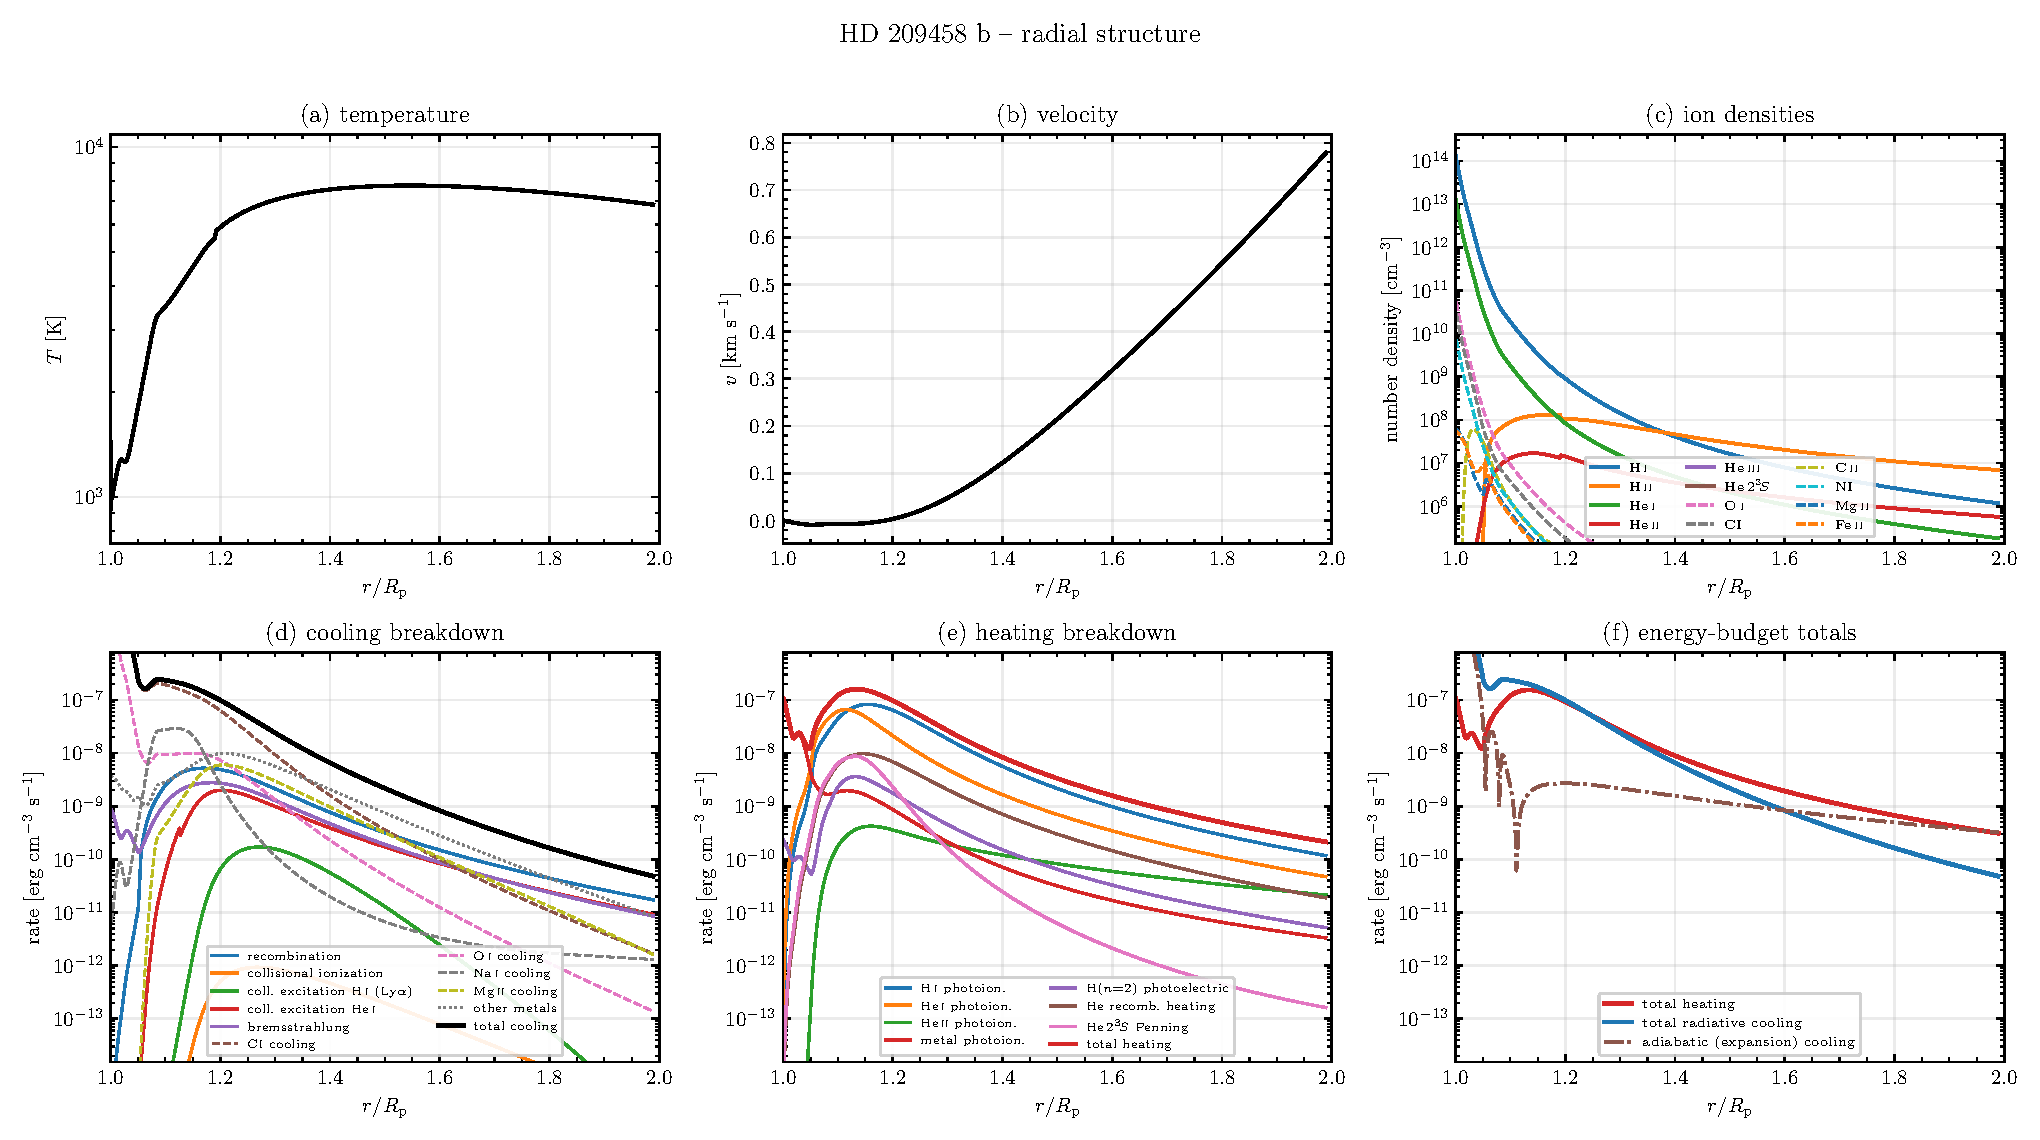
\includegraphics[width=0.92\textwidth]{fig_struct_hd209.pdf}
\caption{Radial structure of the converged HD~209458~b model: (a) temperature, (b) radial
velocity, (c) ion number densities (H and He stages, the metastable $\HeTS$, and the most
abundant metal ions in the wind), (d) the radiative cooling breakdown, (e) the heating
breakdown, and (f) the energy-budget totals. Panel~(d) shows each radiative cooling
channel from the model output, with the collisional-excitation cooling split by absorber
into \mbox{H\,\textsc{i}} (the \Lya-dominated H-line cooling), \mbox{He\,\textsc{i}}, and
\mbox{He\,\textsc{ii}}. Panel~(e) shows the photoionization heating of each absorber
(\mbox{H\,\textsc{i}}, \mbox{He\,\textsc{i}}, \mbox{He\,\textsc{ii}}, $\HeTS$, and the
metals), the excited-hydrogen photoelectric and \Lya\ de-excitation heating, and the
He-recombination and $\HeTS$ Penning heating. Panel~(f) compares the total heating, the
total radiative cooling, and the adiabatic (expansion) cooling computed from the velocity
field. The individual channels in panels (d)--(f) are the ones tabulated in
Table~\ref{tab:energy}. Curves are drawn to the $2\,\Rp$ escape radius. Generated by
\texttt{python/make\_struct\_figures.py}.}
\label{fig:struct_hd209}
\end{figure*}

\subsection{HD~189733~b}
\label{sec:hd189}

For the denser, more strongly bound HD~189733~b the model gives a mass-loss rate of
$\log_{10}(\Mdot/{\rm g\,s^{-1}})=9.04$, the lowest of the four. The thermosphere is hotter
and more compact than that of HD~209458~b, with a temperature maximum of
$\approx1.25\times10^{4}$~K, and the wind is again slow and subsonic through the modeled
region, reaching only $0.5$~km\,s$^{-1}$ at $2\,\Rp$ (Figure~\ref{fig:struct_hd189}).
Hydrogen and helium ionize over a narrow shell just
above the base; the diffusive He/H separation included in this run lets the He/H ratio fall
with altitude.

This is the planet for which the base grid has to be refined. On the default spacing its
base density scale height spans only ${\sim}27$ cells, the least margin of the four, and the
resulting stationary cell-to-cell entropy mode described in Section~\ref{sec:hydro} survives
in the converged state. The model quoted here therefore doubles the base resolution, which
removes the mode from the interior cells; a residual alternating signature remains in the
first two cells above the boundary, where it measures the ghost-to-cell density jump rather
than the entropy mode, and is a documented numerical artifact of the lower boundary rather
than a physical feature. The base temperature this run settles to, ${\sim}490$~K, is set by
where the trapped fine-structure cooling of Section~\ref{sec:cooling} balances the local
metal photoionization heating; the model contains no stellar optical/infrared absorption
and no thermal background, so nothing enforces a floor at the equilibrium temperature for a
layer that has shielded out the XUV.

The synthetic \mbox{He\,10830} depth is $2.5\%$ and \Ha\ is $0.52\%$
(Figures~\ref{fig:transit_he} and~\ref{fig:transit_ha}). The model \mbox{He\,10830} is
about three times deeper than the \citet{Salz2018} detection, which peaks near $0.9\%$, while
sharing the double-peaked triplet shape. Conversely, the clean $\approx2.2\%$ \Ha\ dip
digitized from \citet{Jensen2012} is deeper than the model \Ha, indicating that the $n=2$
population and its \Lya\ pumping in this run under-produce the observed Balmer absorption.
The opposite sign of these two mismatches suggests the discrepancy lies in the excited-state
microphysics rather than in the overall wind density.

\begin{figure*}
\centering
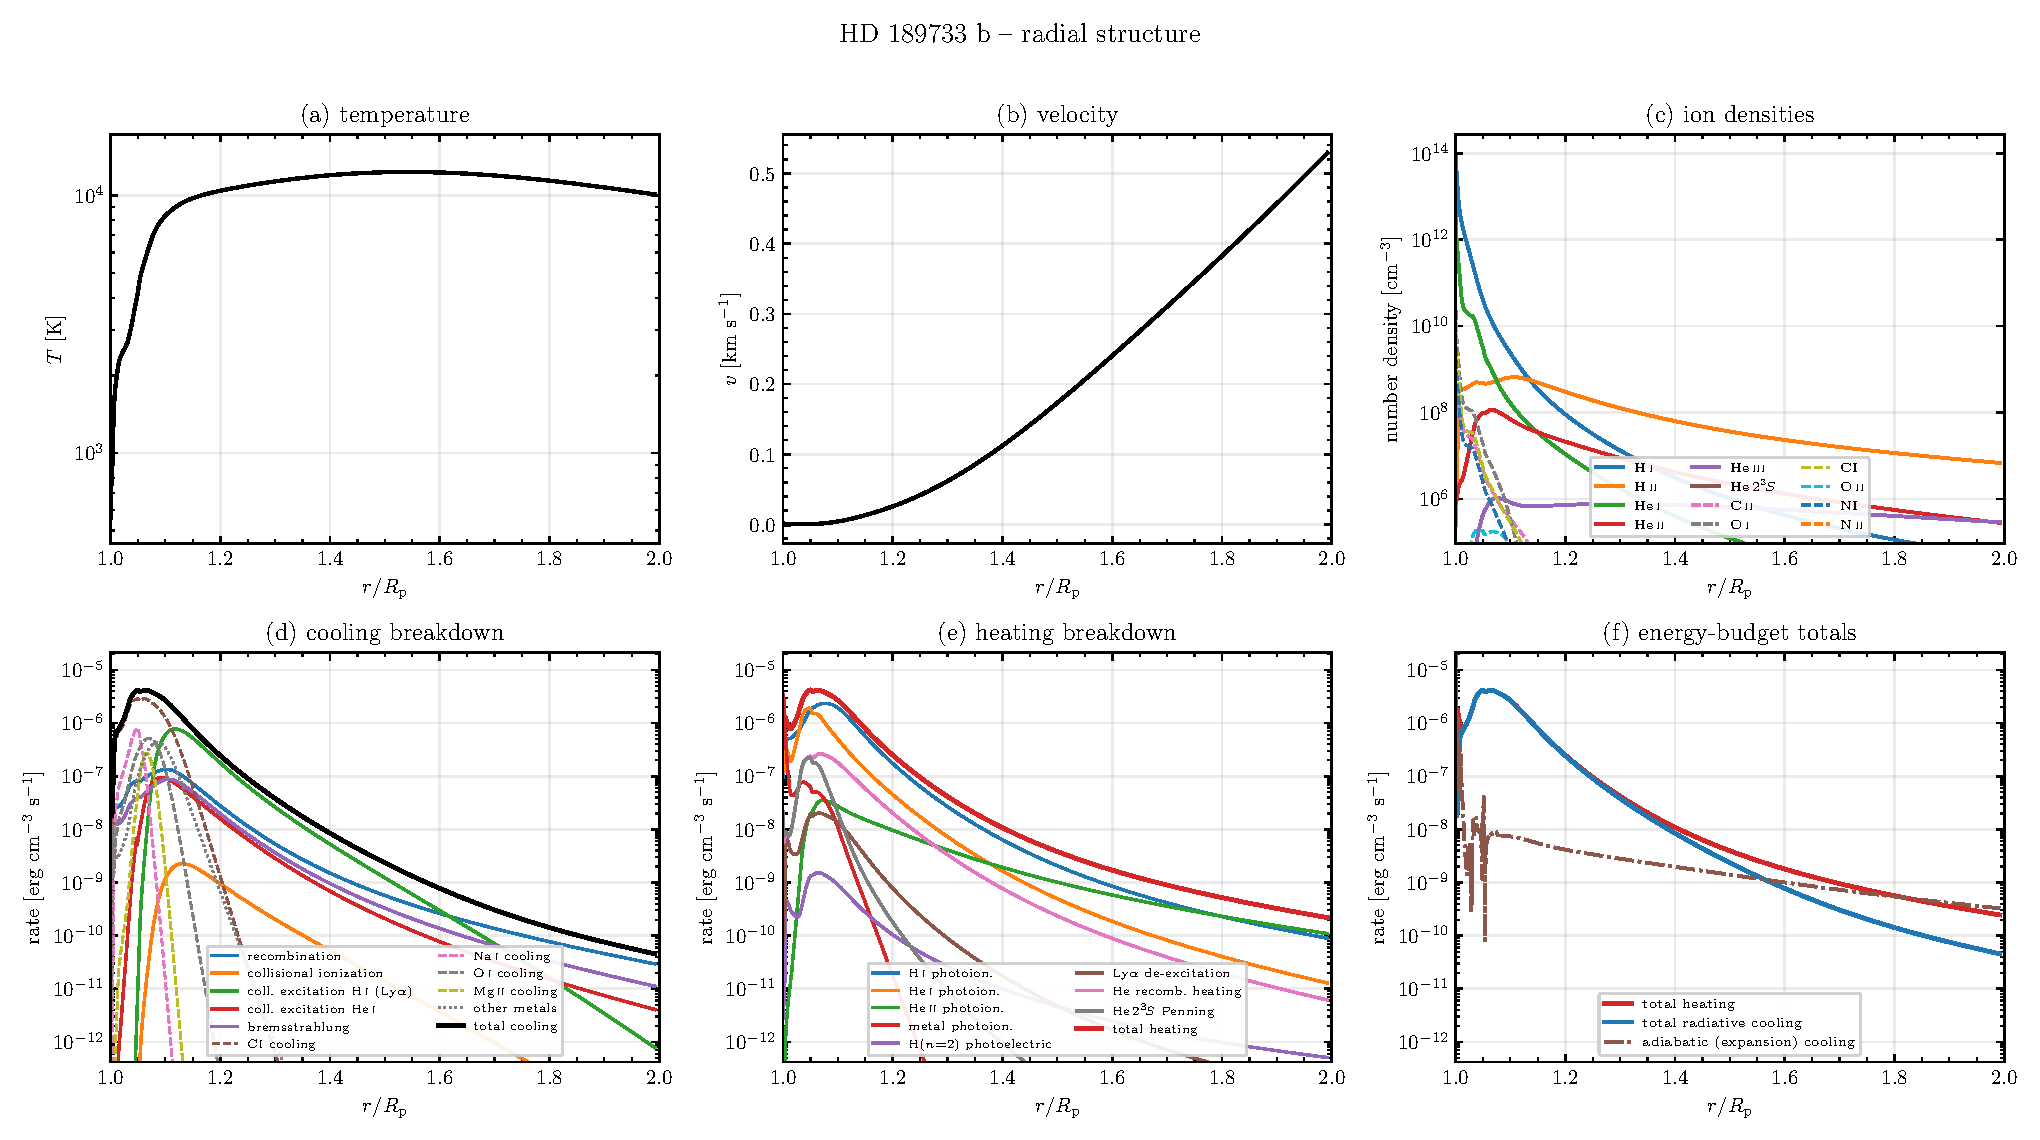
\includegraphics[width=0.92\textwidth]{fig_struct_hd189.pdf}
\caption{Radial structure of the converged HD~189733~b model, as in
Figure~\ref{fig:struct_hd209}. This run includes the diffusive He/H and He/metal
separation. Generated by \texttt{python/make\_struct\_figures.py}.}
\label{fig:struct_hd189}
\end{figure*}

\subsection{WASP-52~b}
\label{sec:wasp52}

WASP-52~b is a low-gravity, strongly irradiated planet, and the model produces a
correspondingly large mass-loss rate of $\log_{10}(\Mdot/{\rm g\,s^{-1}})=11.61$. The
temperature reaches $\approx9.1\times10^{3}$~K and the gas is highly ionized through the
extended thermosphere, which is modeled here on a domain reaching to $10\,\Rp$; the wind
accelerates smoothly, passes $10$~km\,s$^{-1}$ at the $2\,\Rp$ escape radius, and crosses
the sonic point just outside it at $\approx2.2\,\Rp$
(Figure~\ref{fig:struct_wasp52}). The low assumed He/H ratio ($\simeq0.02$) still leaves a
large neutral-hydrogen and metastable-helium column along the extended line of sight.

The resulting transit depths are the largest of the sample: the model \mbox{He\,10830}
triplet reaches $23.5/22.9\%$, \Ha\ $3.5\%$, and \Lya\ is fully saturated near
$100\%$ (Figures~\ref{fig:transit_he}--\ref{fig:transit_lya}). The metal lines are deeper
still, with \mbox{Mg\,\textsc{ii}} at $65.0/57.2\%$ and \mbox{Ca\,\textsc{ii}} at $14.8\%$.
These greatly exceed the measured absorption --- the \citet{Kirk2022}
\mbox{He\,10830} spectrum peaks near $3.6\%$ and the \citet{Chen2020} \Ha\ spectrum is
consistent with a sub-percent signal. The model therefore over-predicts the WASP-52~b line
depths by a factor of several. The most likely contributors are the large radial extent of the
absorbing column on the $10\,\Rp$ domain and the assumed composition; a reduced He/H ratio
and a line of sight truncated nearer the Roche lobe would both lower the predicted depths,
and quantifying this sensitivity is left to future work rather than tuned here. A companion
analysis of the same target separates the two levers. Holding the microphysics and
composition fixed and truncating the line-of-sight integration at the $L_1$ Roche point,
rather than carrying it to $10\,\Rp$, lowers the synthetic \mbox{He\,10830} depth by a
factor of $3$--$10$ on its own, because most of the absorbing column on the extended domain
lies beyond the radius the planet can gravitationally retain. Reducing the helium abundance
from solar to $\mathrm{H/He}\simeq98/2$ then accounts for a further factor of about two, and
the two together reproduce the measured depth. The larger of the two effects is therefore
the domain, which argues that the over-prediction reported here is primarily a geometry
problem, to be addressed with a Roche-lobe truncation of the transit integration rather than
by adjusting the microphysics.

\begin{figure*}
\centering
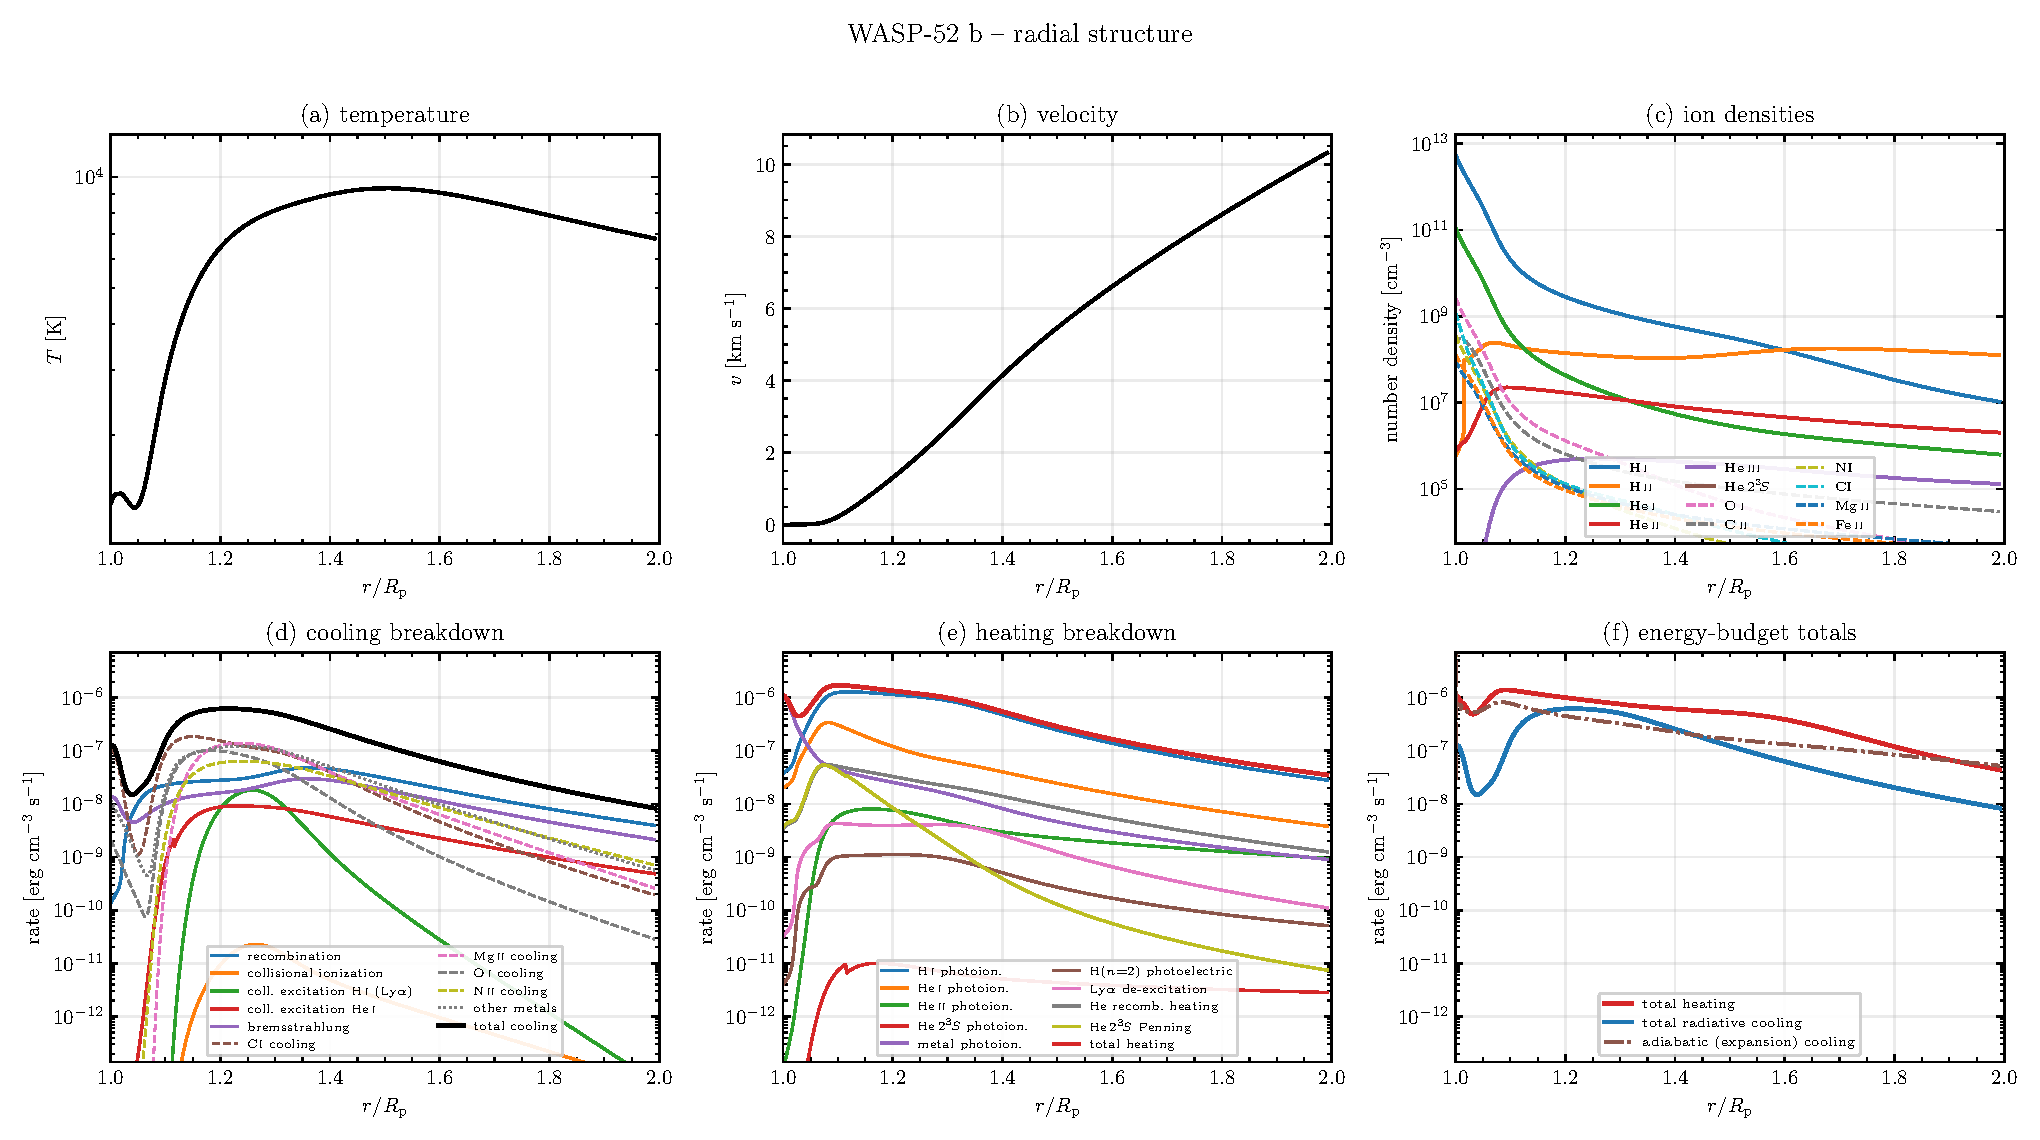
\includegraphics[width=0.92\textwidth]{fig_struct_wasp52.pdf}
\caption{Radial structure of the converged WASP-52~b model, as in
Figure~\ref{fig:struct_hd209}, shown to the $2\,\Rp$ escape radius (the computational
domain extends to $10\,\Rp$). Generated by \texttt{python/make\_struct\_figures.py}.}
\label{fig:struct_wasp52}
\end{figure*}

\subsection{WASP-121~b}
\label{sec:wasp121}

WASP-121~b is the most extreme target, an ultra-hot Jupiter close to Roche-lobe overflow.
The model, computed without diffusive separation, gives a mass-loss rate of
$\log_{10}(\Mdot/{\rm g\,s^{-1}})=13.17$, the highest of the sample. The thermosphere is
very hot --- of order $10^{4}$~K through most of the modeled shell and rising steeply toward
the $1.5\,\Rp$ escape radius --- and the wind reaches $14$~km\,s$^{-1}$ there, crossing the
sonic point at $\approx1.6\,\Rp$, just beyond the escape radius
(Figure~\ref{fig:struct_wasp121}). The gas is strongly ionized, with metal ions
such as \mbox{C\,\textsc{ii}}, \mbox{O\,\textsc{ii}}, and \mbox{N\,\textsc{ii}} carrying an
appreciable fraction of the electrons and contributing to the metal-line cooling. Because
the escape radius lies inside the Roche geometry, the profile near the outer boundary is
sensitive to the domain truncation, and the solution shows a boundary-layer
temperature feature there.

The synthetic depths are the most nearly uniform across lines of the four planets, and
several of them sit at the same value: \mbox{He\,10830} is $3.7\%$, \Ha\ $3.3\%$, \Lya\
$3.7\%$, \mbox{Mg\,\textsc{ii}} $3.8\%$, and \mbox{Ca\,\textsc{ii}} $3.7\%$
(Figures~\ref{fig:transit_he}--\ref{fig:transit_lya}). That common ceiling is geometric
rather than physical. A line whose absorbing column is optically thick all the way to the
edge of the modeled profile blocks the whole annulus between the planet and that edge, so
its depth cannot exceed $(\Rp/\Rstar)^2\,(r_{\rm out}^2-1)$, which is $3.9\%$ here for a
profile ending at $r_{\rm out}=1.61\,\Rp$ on a $1.458\,R_{\odot}$ star. The saturated lines
sit just under that bound. Every one of these depths is therefore a lower bound imposed by
the domain rather than a prediction, and none of them should be read as a measurement of
how much absorption the wind actually produces: what the model establishes on this planet
is that the wind is optically thick in all five lines out to the truncation radius. A
quantitative depth requires a domain carried past the Roche lobe, which is where the
one-dimensional spherical geometry stops being the right description in any case. For the
same reason, the fact that the \mbox{He\,10830} depth exceeds the \citet{Czesla2024}
measurement, which peaks near $2\%$, is not yet evidence of a discrepancy in the
microphysics; we note only that the observed absorption is offset in wavelength relative to
the model line center. That the metal lines saturate at all is consistent with the
metal-rich, highly ionized wind expected for this planet
\citep{Huang2023,Koskinen2022}.

\begin{figure*}
\centering
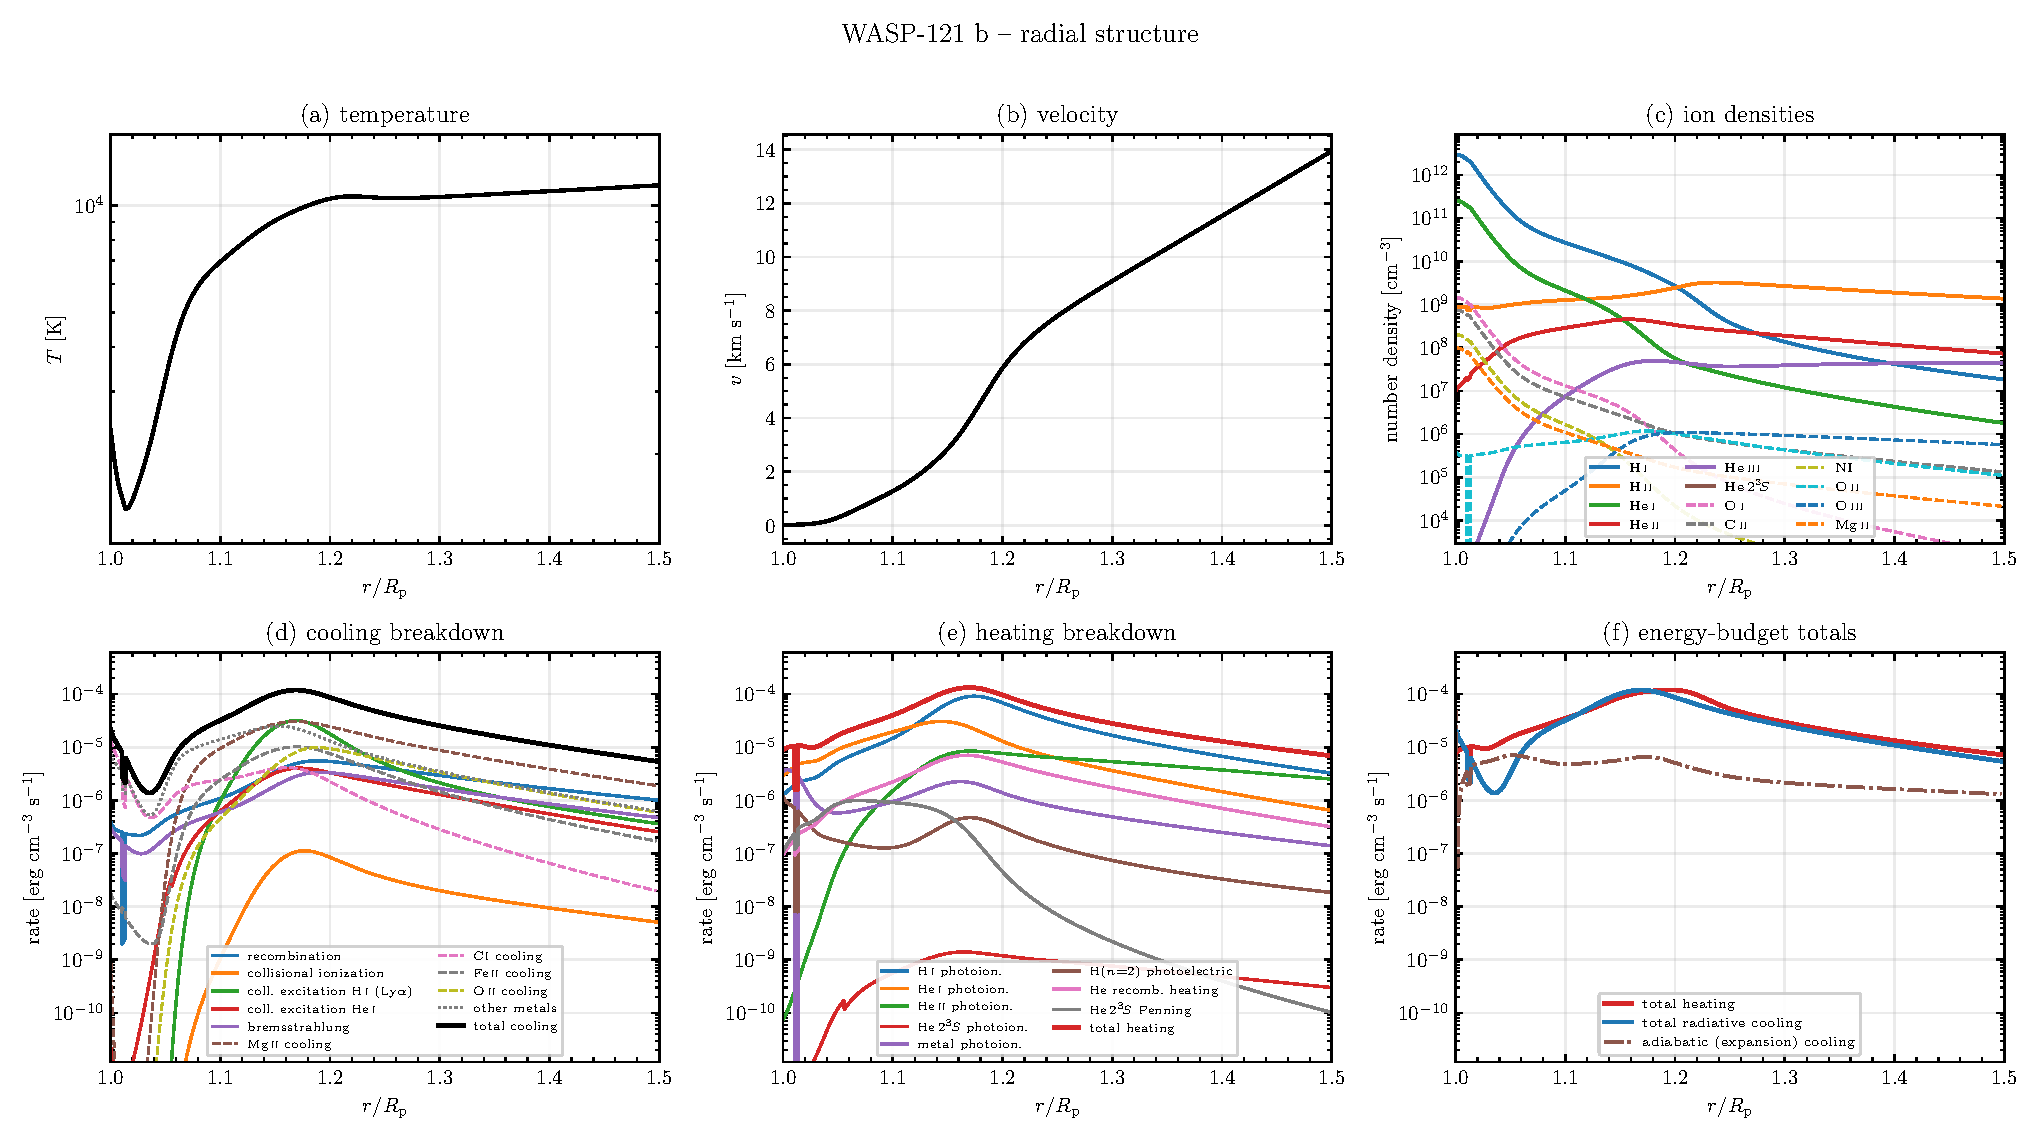
\includegraphics[width=0.92\textwidth]{fig_struct_wasp121.pdf}
\caption{Radial structure of the WASP-121~b model (no diffusive separation),
as in Figure~\ref{fig:struct_hd209}, shown to the $1.5\,\Rp$ escape radius. The temperature
panel is clipped to a robust upper percentile so the boundary-layer feature near the escape
radius does not dominate the scale. Generated by
\texttt{python/make\_struct\_figures.py}.}
\label{fig:struct_wasp121}
\end{figure*}

\begin{figure*}
\centering
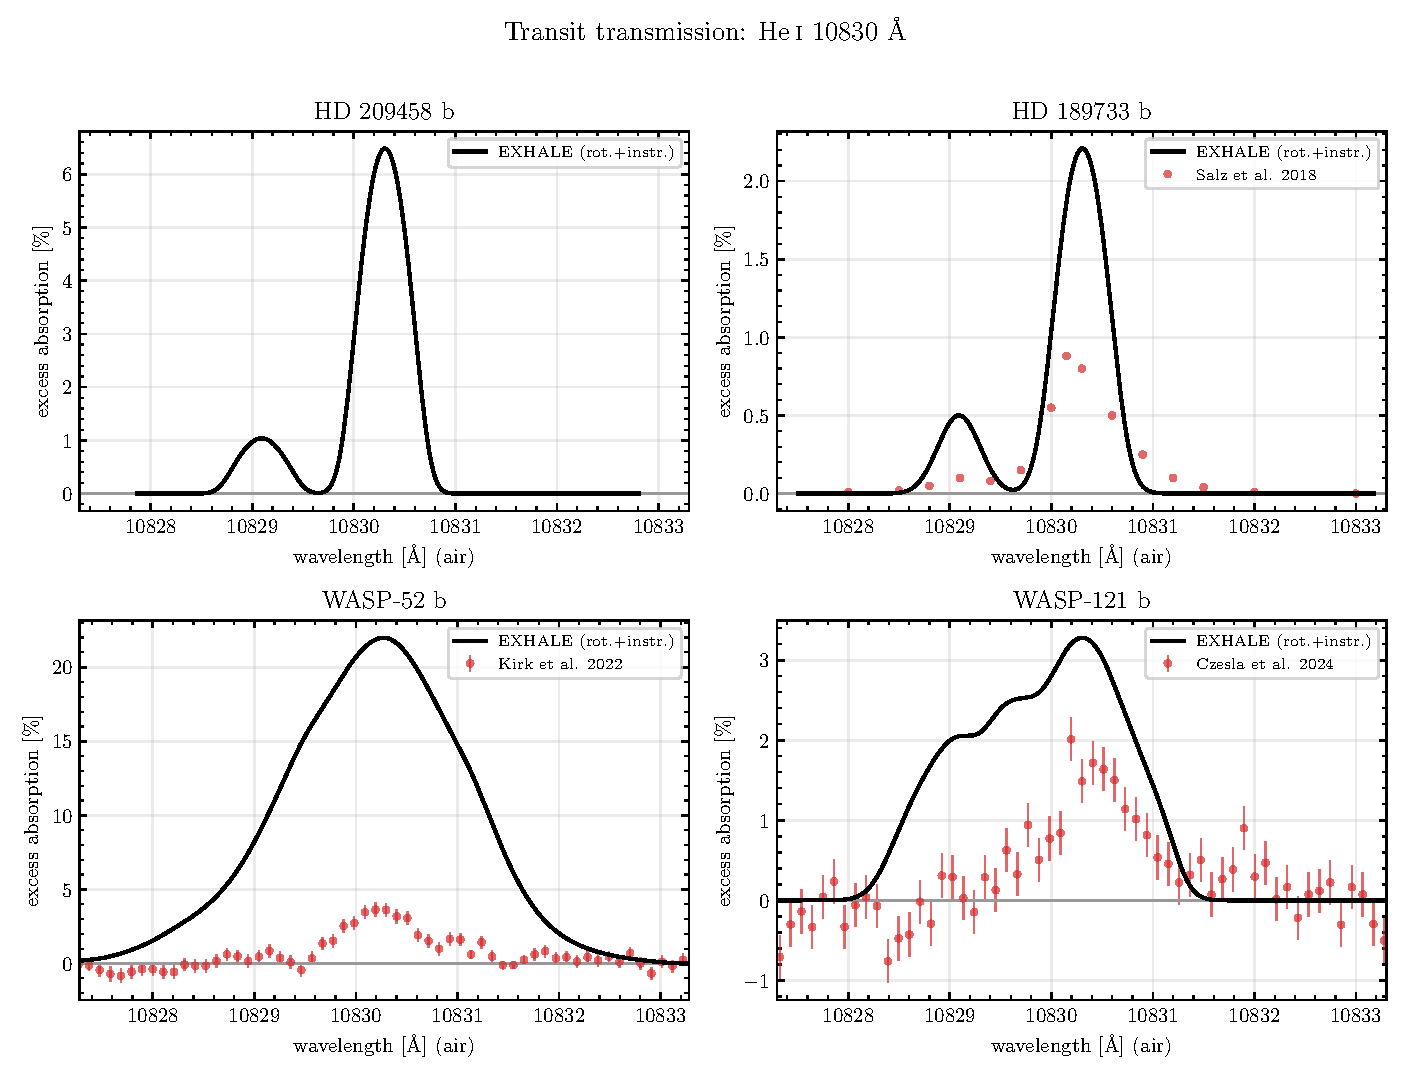
\includegraphics[width=0.92\textwidth]{fig_transit_He10830.pdf}
\caption{Synthetic \mbox{He\,\textsc{i}} 10830 transit spectra (rotation- and
instrument-convolved) for the four planets, compared with published observations where
available: \citet{Salz2018} for HD~189733~b, \citet{Kirk2022} for WASP-52~b, and
\citet{Czesla2024} for WASP-121~b. All curves are shown as excess absorption, $(1-T)$ in
percent; each observation is converted to this common axis from its native convention
(dF/F, excess-absorption percent, or normalized in/out flux). Generated by
\texttt{python/make\_transit\_figures.py}.}
\label{fig:transit_he}
\end{figure*}

\begin{figure*}
\centering
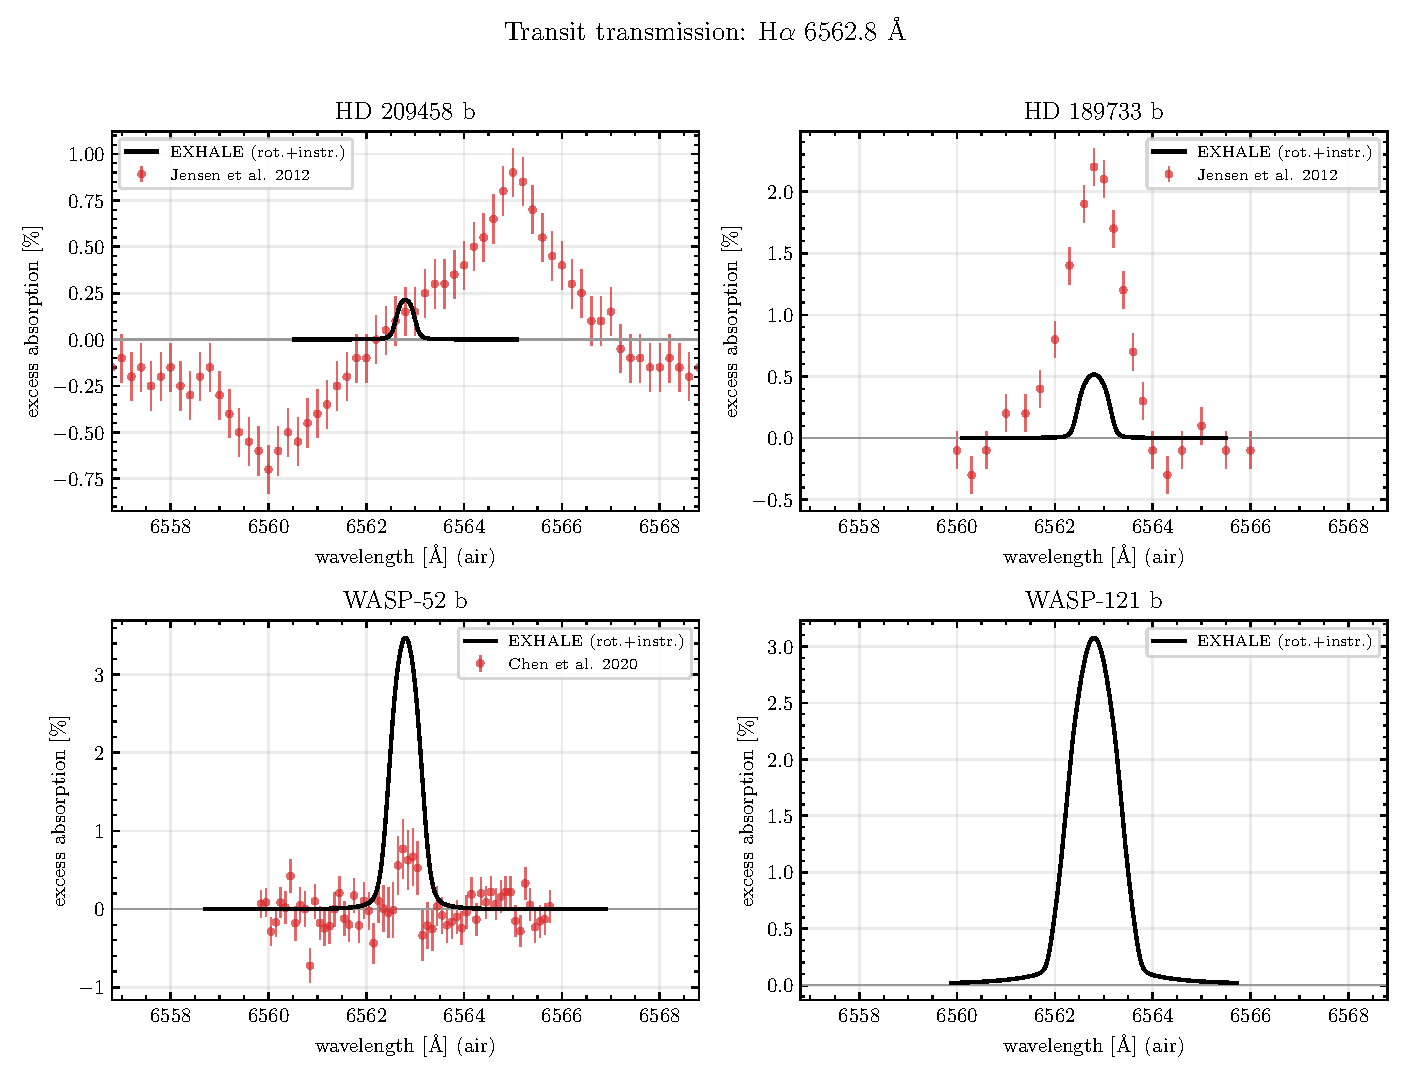
\includegraphics[width=0.92\textwidth]{fig_transit_Halpha.pdf}
\caption{Synthetic \Ha\ transit spectra, as in Figure~\ref{fig:transit_he}, compared with
the digitized \citet{Jensen2012} traces (HD~209458~b and HD~189733~b) and the
\citet{Chen2020} ESPRESSO spectrum (WASP-52~b). Generated by
\texttt{python/make\_transit\_figures.py}.}
\label{fig:transit_ha}
\end{figure*}

\begin{figure*}
\centering
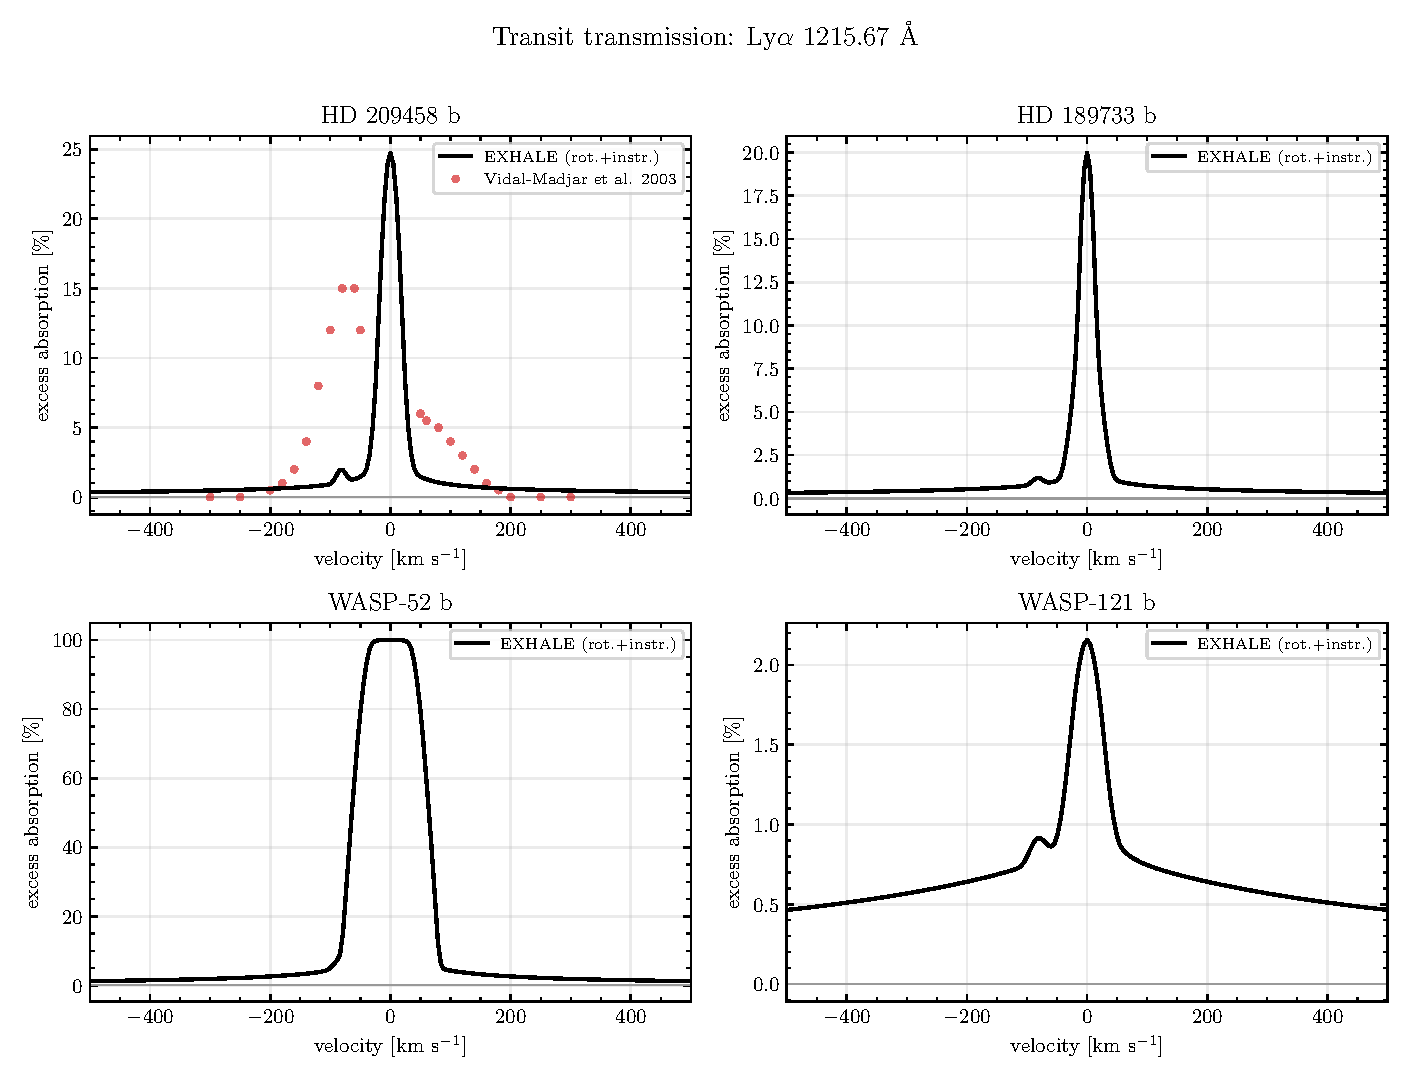
\includegraphics[width=0.92\textwidth]{fig_transit_Lya.pdf}
\caption{Synthetic \Lya\ transit spectra on a velocity axis, as in
Figure~\ref{fig:transit_he}. The HD~209458~b panel overplots the wing profile of
\citet{VidalMadjar2003}; the line core (roughly $\pm40$~km\,s$^{-1}$) is omitted in the
data because of interstellar and geocoronal absorption. No \Lya\ measurements are available
for the other three planets. Generated by \texttt{python/make\_transit\_figures.py}.}
\label{fig:transit_lya}
\end{figure*}

%=====================================================================
\section{Summary}
\label{sec:summary}
%=====================================================================

We have described \EXHALE, a one-dimensional multi-frequency photoionization--hydrodynamics
model for escaping exoplanet atmospheres. Building on the \ATES\ Godunov hydro core,
\EXHALE\ adds a coupled H/He/metal ionization network with Badnell recombination, Voronov
collisional ionization, and Kingdon \& Ferland charge exchange; CHIANTI metal-line
cooling; the $\HeTS$ metastable triplet; the non-LTE $n=2$ hydrogen population with an
in-line \Lya\ escape-probability field; optional diffusive He/H separation; a direct JFNK
steady-state solver; and a tiered lower-atmosphere coupling. Applied to HD~209458~b,
HD~189733~b, WASP-52~b, and WASP-121~b, the model produces mass-loss rates and synthetic
\mbox{He\,10830}, \Ha, \Lya, and metal-line transit spectra for direct comparison with
observations. Across the four benchmarks the model gives mass-loss rates of
$\log_{10}(\Mdot/{\rm g\,s^{-1}})=9.31$ (HD~209458~b), $9.04$ (HD~189733~b), $11.61$
(WASP-52~b), and $13.17$ (WASP-121~b), each converged with the steady-state solver rather
than stopped on the mass-flux criterion, and synthetic line depths that match the order of
magnitude of the measured \mbox{He\,10830}, \Ha, and \Lya\ absorption on HD~209458~b and
HD~189733~b, while over-predicting the WASP-52~b depths and saturating against the domain
truncation on WASP-121~b. The priorities these point to are the composition and the
line-of-sight domain, a transit geometry carried past the Roche lobe for the most extended
winds, and the excited-state microphysics behind the opposite-sign HD~189733~b
\mbox{He\,10830} and \Ha\ mismatches.

\begin{acknowledgments}
%% PLACEHOLDER: acknowledgments, funding, facilities.
\end{acknowledgments}

\software{\texttt{EXHALE}, \texttt{ATES} \citep{Caldiroli2021},
  \texttt{VULCAN} \citep{Tsai2017}, \texttt{LaRT} \citep{SeonKim2020},
  \texttt{p-winds} \citep{dosSantos2022}, CHIANTI \citep{Dere1997,DelZanna2021}}

\bibliographystyle{aasjournalv7.1}
\bibliography{ms}

\end{document}
